\documentclass[12pt]{article}

\usepackage[utf8]{inputenc}
\usepackage[T1]{fontenc}
\usepackage{graphicx}
\usepackage{tikz}
\usepackage{xcolor} 

\usetikzlibrary{chains,fit,shapes,decorations.pathreplacing}
\edef\sizetape{0.6cm} 
\tikzstyle{tmtape}=[draw,minimum size=\sizetape]
\definecolor{lightgrey}{RGB}{192,192,192}

\newcommand{\TBM}{Turbo\_BM }

\begin{document}
\title{Algorytm \TBM}
\author{Adrian Siwiec}
\maketitle

\section*{Opis Algorytmu.}
Algorytm \TBM jest modyfikacją algorytmu Boyera-Moore'a, która zużywa tylko stałą dodatkową pamięć oraz przyspiesza złożoność pesymistyczną do $2n$. Nie będziemy wykonywać żadnego dodatkowego preprocessingu -- tak jak w oryginalnym algorytmie korzystać będziemy z tablicy BM obliczonej dla wzorca.
  
Sam pomysł algorytmu \TBM jest bardzo prosty -- podczas skanowania będziemy zapisywać jedno podsłowo wzorca, o którym wiemy że pasuje do tekstu na obecnej pozycji. Dzięki temu możemy pominąć ten fragmeny przy sprawdzaniu dopasowania, oraz w przypadku jego braku możemy wykonać tzw. \emph{Turbo-shift}.

Niech $x$ będzie najdłuższym sufixem, który pasuje do tekstu na danej pozycji wzorca, $a$ będzie pierwszą literą wzorca która nie pasuje, a niech $y$ ($memory$) będzie poprzednio zapamiętanym podsłowem, które również pasuje do wzorca (patrz fig. \ref{turboshift}). Załóżmy również, że $x$ i $y$ są rozłączne i $y$ jest dłuższy od $x$. Po wykonaniu Turbo-shift zapominamy o $y$ (patrz kod \emph{boyer\_moore\_turbo}), więc w poprzednim kroku wykonaliśmy zwykłe przesunięcie (zgodnie z tablicą $BM$), znane z algorytmu Boyera-Moore'a. W tej sytuacji $ax$ jest sufixem $y$, oraz litery $a$ i $b$ tekstu są o siebie oddalone o $|y|$. Ale suffix $y\ldots x$ ma okres długości $|y|$ (z definicji $BM$). Możemy więc przesunąć wzorzec o $|y| - |x|$ do przodu i to właśnie przesunięcie nazywać będziemy \emph{Turbo-shift}.

% Spójrzmy na kod algorytmu \TBM:
% \begin{code}
% 	\captionof{listing}{Algorytm Boyera-Moore'a}
%   \begin{minted}{python}
%     import numpy as np
%   \end{minted}
% 	\label{alg:exact-string-matching-boyer-moore}
% \end{code}

\begin{figure}[h]
	\centering
	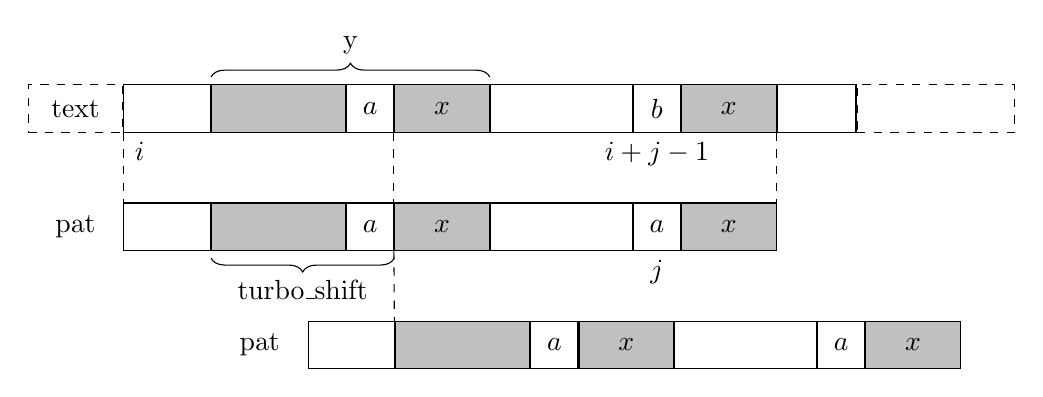
\begin{tikzpicture}
		\begin{scope}[shift={(0,0)}, start chain=1 going right,node distance=0mm]
			\node [on chain=1,tmtape, minimum width=1.2cm, dashed] {text};
			\node [on chain=1,tmtape, minimum width=1.1cm, label={[xshift=-.35cm]below:$i$}] (textStart) {};
			\node [on chain=1,tmtape, minimum width=1.7cm, fill=lightgrey] {};
			\node [on chain=1,tmtape] (textA) {$a$};
			\node [on chain=1,tmtape, minimum width=1.2cm, fill=lightgrey]  {$x$};
			\node [on chain=1,tmtape, minimum width=1.8cm] (textMemEnd) {};
			\node [on chain=1,tmtape, label={below:$i+j-1$}] (textMatchStart) {$b$};
			\node [on chain=1,tmtape, minimum width=1.2cm, fill=lightgrey] (textEnd) {$x$};
			\node [on chain=1,tmtape, minimum width=1cm] (textMatchEnd) {};
			\node [on chain=1,tmtape, minimum width=2cm, dashed] {};
						
			\draw[decorate,decoration={brace,amplitude=5pt,raise=.4cm}] (textStart) -- (textMemEnd) node [midway, yshift=.8cm] {y};
						
			% \draw[decorate,decoration={brace,amplitude=5pt,raise=.4cm}] (textMatchStart) -- (textMatchEnd) node [midway, yshift=.8cm] {match};
		\end{scope}
		\begin{scope}[shift={(0,-1.5)}, start chain=1 going right,node distance=0mm]
			\node [on chain=1,tmtape, minimum width=1.2cm, draw=none] {pat};
			\node [on chain=1,tmtape, minimum width=1.1cm] (patStart) {};
			\node [on chain=1,tmtape, minimum width=1.7cm, fill=lightgrey] {};
			\node [on chain=1,tmtape] (patA) {$a$};
			\node [on chain=1,tmtape, minimum width=1.2cm, fill=lightgrey] (patAEnd) {$x$};
			\node [on chain=1,tmtape, minimum width=1.8cm] {};
			\node [on chain=1,tmtape, label={below:$j$}] {$a$};
			\node [on chain=1,tmtape, minimum width=1.2cm, fill=lightgrey] (patEnd) {$x$};
						
			\draw[decorate,decoration={brace,amplitude=5pt,mirror,raise=.4cm}] (patStart) -- (patAEnd) node [midway, yshift=-.8cm] {turbo\_shift};
		\end{scope}
				
		\draw[dashed,transform canvas={xshift=0.3cm}] (textA) -- (patA);
		\draw[dashed,transform canvas={xshift=-0.55cm}] (textStart) -- (patStart);
		\draw[dashed,transform canvas={xshift=0.6cm}] (textEnd) -- (patEnd);
				
		\begin{scope}[shift={(2.34,-3)}, start chain=1 going right,node distance=0mm]
			\node [on chain=1,tmtape, minimum width=1.2cm, draw=none] {pat};
			\node [on chain=1,tmtape, minimum width=1.1cm] (pat2Start) {};
			\node [on chain=1,tmtape, minimum width=1.7cm, fill=lightgrey] {};
			\node [on chain=1,tmtape] (pat2A) {$a$};
			\node [on chain=1,tmtape, minimum width=1.2cm, fill=lightgrey] {$x$};
			\node [on chain=1,tmtape, minimum width=1.8cm] {};
			\node [on chain=1,tmtape] {$a$};
			\node [on chain=1,tmtape, minimum width=1.2cm, fill=lightgrey] (pat2End) {$x$};
		\end{scope}
				
		\draw[dashed,transform canvas={xshift=0.3cm}] (patA) -- (3.75cm,-2.7cm);
	\end{tikzpicture}
		
  \caption{Turbo-shift}
  \label{turboshift}
\end{figure}
  
\section*{Analiza złożoności.}

\end{document}